\chapter[Chiral--Fractal Temporal Topology]{Chiral--Fractal Temporal Topology as a Derived-Property Gate}
The Neutrinotime line motivates a fractal--chiral temporal topology as a comparison target. In the present derivation, the target is decomposed into independently testable quantities:
\[
I_{\rm top}[\Gamma],\qquad \chi[\Gamma],\qquad D_F[\Gamma].
\]
These denote, respectively, a topological invariant, a signed chirality/orientation observable, and a fractal-scaling observable of an orbit or invariant set \(\Gamma\).

A minimal chirality candidate is a signed holonomy,
\[
\chi[C]=\operatorname{sgn}\!\left(\oint_C A\right),
\]
whenever the dynamical state bundle supplies an admitted connection \(A\). Orientation reversal must reverse the sign of \(\chi\) while declared non-chiral invariants remain unchanged.

Fractality is measured prospectively from the derived tensor--scalar dynamics through \(D_F\), a renormalization relation, a Lyapunov diagnostic, or another explicit scaling test. A linear Kähler control supplies the non-fractal reference class.

The relation between event-localized NOW and a dynamical bifurcation locus remains an open bridge. They are maintained as separate typed objects until an equivalence theorem or prospective experiment closes that dependency.

\section{Visual intuition for chirality and event structure}
The schematic rendering in Figure~\ref{fig:temporal-ribbon-3d} shows a single trajectory lifted over an informational landscape, making visible the joint role of orbital phase and informational descent. Figure~\ref{fig:event-measure} then shows a schematic discrete event measure extracted from an evolving informational signal.
\begin{figure}[H]
  \centering
  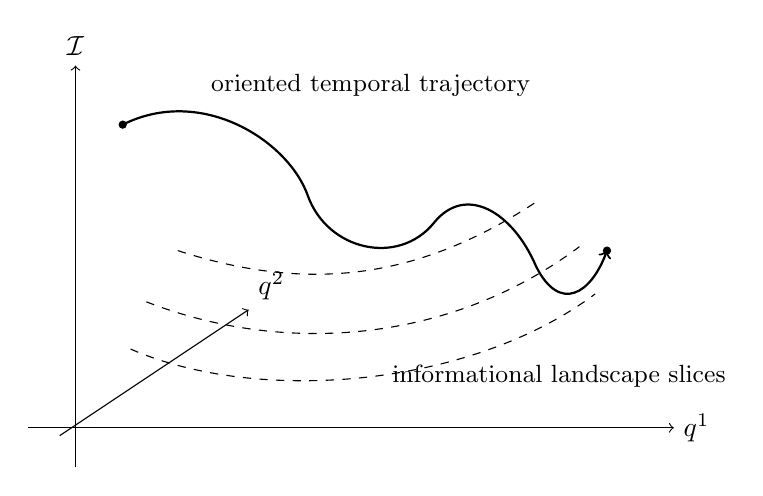
\begin{tikzpicture}[scale=1.0]
    \draw[->] (-4.0,-1.9) -- (4.2,-1.9) node[right] {$q^1$};
    \draw[->] (-3.4,-2.4) -- (-3.4,2.7) node[above] {$\mathcal I$};
    \draw[->] (-3.6,-2.0) -- (-1.2,-0.4) node[above right] {$q^2$};
    \draw[dashed] (-2.7,-0.9) .. controls (-1.1,-1.6) and (1.6,-1.4) .. (3.2,-0.2);
    \draw[dashed] (-2.5,-0.3) .. controls (-0.7,-1.0) and (1.4,-0.8) .. (3.0,0.4);
    \draw[dashed] (-2.1,0.35) .. controls (-0.4,-0.2) and (1.0,0.0) .. (2.5,1.0);
    \draw[->,thick]
      (-2.8,1.95)
      .. controls (-1.8,2.45) and (-0.7,1.75) .. (-0.45,1.05)
      .. controls (-0.20,0.35) and (0.70,0.15) .. (1.15,0.70)
      .. controls (1.55,1.20) and (2.15,0.85) .. (2.45,0.15)
      .. controls (2.75,-0.45) and (3.15,-0.20) .. (3.35,0.35);
    \fill (-2.8,1.95) circle (1.5pt);
    \fill (3.35,0.35) circle (1.5pt);
    \node[font=\small,anchor=west] at (-1.8,2.45) {oriented temporal trajectory};
    \node[font=\small,anchor=west] at (0.5,-1.25) {informational landscape slices};
  \end{tikzpicture}
  \caption{Schematic lifted slice of temporal evolution on the Kähler informational landscape. The vertical coordinate represents the informational functional $\mathcal{I}$ along an oriented trajectory.}
  \label{fig:temporal-ribbon-3d}
\end{figure}
\begin{figure}[H]
  \centering
  \begin{tikzpicture}[x=0.92cm,y=1.0cm]
    \draw[->] (0,0) -- (11.2,0) node[right] {$\lambda$};
    \draw[->] (0,-0.2) -- (0,3.0) node[above] {event weight};
    \draw[dashed] (0,1.0) -- (10.7,1.0) node[right,font=\small] {reference level};
    \foreach \x/\h in {0.7/0.35,1.5/0.75,2.4/0.45,3.2/1.55,4.0/0.65,5.1/2.35,6.0/0.55,6.9/1.25,7.8/0.50,8.9/1.90,9.8/0.70}
      \draw[thick] (\x,0) -- (\x,\h);
    \foreach \x/\h in {3.2/1.55,5.1/2.35,6.9/1.25,8.9/1.90}
      \fill (\x,\h) circle (1.8pt);
    \node[font=\small,anchor=west] at (3.35,2.65) {localized event support};
  \end{tikzpicture}
  \caption{Schematic discrete event measure on the ordering parameter. Selected localized peaks illustrate the event-support coordinate used to compare temporal evolution with NOW localization.}
  \label{fig:event-measure}
\end{figure}
